%
%	Begrifflichkeiten
%

\pagebreak
\section{Data Sources and Research Methods}

\onehalfspacing

\subsection{The Blog}

The blog in question is my personal \href{https://chfrank.net/wordpress}{web log} that I started a couple of years ago, initially on the now-defunct Google+ platform. It's now on a hosted WordPress instance provided by a local service provider running on a web server farm in Strasbourg. A move from Google+ to Blogger instead of WordPress might have been the more comfortable choice and allowed for more consistency; however, I made a clean break between the hosting platforms. The original Google+ data is lost. I maintain some Google+ connections on Diaspora*, though.

I use the blog to complement my other social media whenever I feel the need to express myself in slightly longer texts. I try to post at least once per week and cross-post the blog entries to my other channels, private and professional; for small essays, I use Medium to publish them.

Although I do cross-post, I never duplicate entries, and thus there is no dilution of data; the data from every post is unique, and all content is only published once.

During the current and past COVID-19 lockdowns, I wrote a running week-by-week commentary, affecting the traffic analysis outcome, as we'll see later.

\subsection{Plausible}

The data I'll be using was collected using GDPR-compliant web analytics by Plausible, a lightweight and open-source website analytics tool. Plausible provides an easy-to-use webhook to integrate its analytics with almost any kind of website framework; it is ad-free and offered as Software-as-a-Service with a subscription model.

Plausible does not use any tracking cookies and claims to be fully compliant with GDPR, CCPA, and PECR. In addition to the web analytics data, I will complement Plausible's data with additional data from the blog.

\begin{figure}[H]
\centering
\caption {Plausible Summary}
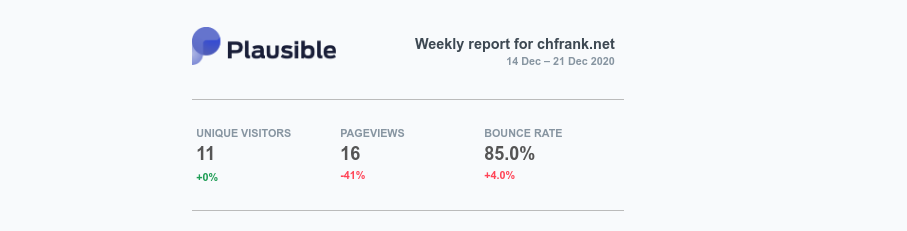
\includegraphics[width=\linewidth]{images/plausible.png}
\label{fig:plausibleSummary}
\end{figure}

In a previous paper, I have covered Plausible in more detail and compared it with other web analytics tools\footnote{See \textit{Frank, C. (2020)}: Usefulness of open-source tools for web analytics in E-Marketing.\cite{previousPaper}}; I will not go any further into details of the tool itself in this paper.

In case you're interested, you can find up-to-date raw web traffic data from the blog here: \href{https://plausible.io/chfrank.net}{Plausible Analytics}.

\subsection{Count}

To analyze and visualize the data, I'll be using data notebooks from Count. Like Jupyter notebooks that combine (Python) Code and Text, the data notebooks combine (SQL) Data and Text in a pretty ingenious way. Data notebooks support data-driven decision making, and they are currently in open beta.\footnote{See \textit{Count.co (2020)}: About Count.\cite{aboutCount}}

\subsection{Web Traffic KPIs}

In marketing categories, a blog belongs to inbound marketing, as it tries to offer engaging content and create value for the visitors but does not reach out by itself. 

Unlike outbound email campaigns, for example, that ask the visitor to view a particular website, a blog relies on its content and the willingness of the visitor to actively choose the site for a visit, for example, by being pointed to a post from a Google search result or a tweet.

In WordPress, there is an option to subscribe to a blog to get a notification on new posts; WordPress also provides the ability to subscribe to a blog's RSS feed. Even though, as this requires active user interaction and interest, blogs are considered an inbound channel.

In a recent paper on inbound marketing, Yvonne Romes identifies a couple of important KPIs for inbound marketing, a couple of which I will summarize here based on her paper:\footnote{See \textit{Romes, Y. (2020)}: 10 Inbound KPIs, die jetzt auch Personaler kennen sollten.\cite{inboundKPI}}

\begin{itemize}
\item Page Views
\item Bounce Rate
\item Visit Duration
\item Unique Visitors
\end{itemize}

Page Views is the number of clicks a specific page has received; on a blog, more page views indicate more engaging content.

Bounce Rate describes the rate of users that leave the site without selecting another link; a high bounce rate can indicate a lack of engaging or interesting content.

Visit Duration is the amount of time a unique visitor spends on the website; for a blog that mainly offers content to read, a longer duration most likely indicates higher engagement.

A unique visitor is a visitor that can be differentiated from another visitor. Unlike many other platforms, Plausible does not use tracking cookies to identify individual visitors but relies on publicly available information, such as an IP address, to differentiate them. Even though the metric is less accurate with Plausible than with other platforms, it's still an important metric, and as before, on a blog, more visitors usually indicate higher engagement.

In this paper, these are the four metrics that I will focus on.

\subsection{Statistical Methods}

I will base the analysis on the excellent work and great documentation available at Towards Data Science, a platform on Medium to exchange ideas and to expand the understanding of data science.\footnote{See \textit{TDS Editors (2018)}: About Towards Data Science.\cite{aboutTDS}}

Vital elements in data science are statistics and linear algebra.

"From an academic perspective, understanding linear algebra is paramount to having a strong knowledge of specific topics within computer vision and deep learning."\footnote{\textit{Alake, R. (2020)}: 6 Questions Asked By Machine Learning Enthusiasts.\cite{sixQuestions}}

An excellent reference for using linear algebra in data science and machine learning is the book "Mathematics for Machine Learning" by Marc Peter Deisenroth, A. Aldo Faisal, and Cheng Soon Ong.\footnote{See \textit{Deisenroth, M.P. (2020)}: Mathematics for Machine Learning.\cite{mathematicsML}}

This paper will stay relatively simple and only look at two-dimensional data to identify possible correlations between measurements. I am acutely aware of the fact that "correlation does not imply causation"\footnote{See \textit{Singh, S. (2020)}: Why correlation does not imply causation.\cite{correlateCause}} and will make sure that our findings match real-world scenarios and experiences.

Statistics is the other bedrock of data science. In this paper, I will measure central tendency through arithmetic mean, median, and mode of our data.\footnote{See \textit{Yıldırım, S. (2020)}: 10 Must-Know Statistical Concepts for Data Scientists.\cite{bedrockScience}}

The actual data set is small, as the blog does not have a lot of traffic, so any method that relies on a high number of data points will not work. For the analysis and predictions of future performance, I will depend mainly on visualization techniques, tables, and verbal interpretation of the data.

\subsection{Sentiment Analysis}

The blog already has categories for its content, so there's no need to extract content information from the posts to categorize them manually. There is, however, no information in the blog data in regards to the sentiment of the post.

Especially concerning the current pandemic, I think it can make a lot of difference if a blog post is either upbeat or somewhat fatalistic, so I will attempt to identify the individual entries' sentiment.

To do this, I will use sentiment analysis. Sentiment analysis is a technique from the field of Natural Language Processing and fits into Contextual Semantic Search. 

Sentiment analysis aims to identify a text message's sentiment as either positive, negative, or neutral.\footnote{See \textit{Gupta, S. (2018)}: Sentiment Analysis: Concept, Analysis and Applications.\cite{sentimentAnalysis}} With the categories already present, there's no need to go deeper and add intent or context to the analysis; it will suffice to enrich the post data with sentiment information.

There are several ready-made sentiment analysis libraries available for both R and Python. Since I am a bit more familiar with Python and functional programming than with R, I will concentrate on using Python in the next chapters.
